\paragraph{Rationale}
Because the editors center around a tree structure, a clear understanding of trees is helpful.

\paragraph{Trees}
A \textit{tree} is a data structure.
The tree is composed of \textit{nodes}, and one node is designated as the \textit{root node} node or \textit{tree root}.
Each node can have zero or more \textit{children} nodes, and one \textit{parent} node.
The root node does not have a parent.
When representing the tree as code, it is possible to omit either the parent or child relationship in a node, making the parent or child implicit.
The relationship can still be found, by \textit{traversing} the tree.
Traversing means to visit every node it the tree by following the parent or child relationships.
Nodes that are children of the same parent are called \textit{siblings}, and parents of parents are called \textit{grandparents}.

\paragraph{Visualizing trees}
There are many ways to present trees to humans.
Two common approaches are \textit{hierarchy} and \textit{diagram}.\\

In a hierarchy, the parent is presented as a row, and its children on separate rows below (see \cref{sfig:tree-visualized-hierarchy}).
The children are often indented as well, and possibly connected with dots or lines to the parent.\\

In a diagram, nodes are often displayed as a circle or box (see \cref{sfig:tree-visualized-diagram}).
The parent is displayed above its children, and the children are aligned on the same row.
The parent-child relationship is shown as a line or arrow, connecting the parent to the child.

\begin{figure}[htbp]
    \centering
    \begin{subfigure}[b]{.45\textwidth}
        \centering
        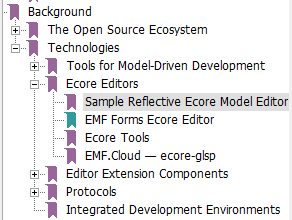
\includegraphics[width=\textwidth]{figures/tree-hierarchy.png}
        \caption{A tree visualized as a hierarchy. The top node is the root.}\label{sfig:tree-visualized-hierarchy}
    \end{subfigure}
    \hfill
    \begin{subfigure}[b]{.45\textwidth}
        \centering
        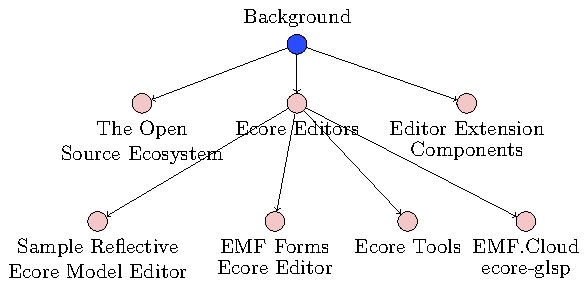
\includegraphics[width=\textwidth]{figures/tree-diagram.pdf}
        \caption{A tree visualized as a diagram. The blue node at the top is the root.}\label{sfig:tree-visualized-diagram}
    \end{subfigure}
    \caption[Tree Structure Visualizations]{A tree visualized as a hierarchy and diagram. The labels are section titles of \cite{rekstadModelingEnvironmentCloud2020}, as an example.}\label{fig:tree-visualized}
\end{figure}

\paragraph{Nodes}
The tree is more useful when the nodes have properties.
The minimum property is children or parent.
But a useful property is a name, label or id, with regards to presenting the tree to a human.
There may be properties on the relationships between a node and its children, but these may be hard to present visually in hierarchy-type visualizations.
For a diagram type visualization, the properties may be presented as labels on the edge.

\paragraph{Mapping to trees}
A data structure can be mapped to a tree if it has separate objects with a references, containment or aggregation relationship.
The references can not be circular (where a node has a child which is also a parent or grandparent etc.).
There can be different ways to map to a tree, depending on what properties are used (or not used).
The labels can also come from various object properties, be derived from them or combine multiple properties into one label.

\paragraph{Editing a tree}
Common operations on trees either modify the structure, or modify the properties of a node.
Structural modifications can be to add a new child, to delete a child, or to move a child from one parent to another.
Nodes can be copied, and pasted on the same parent or other parents, or themselves.
Less common operations are inserting a new node between a parent and child, turning the latter into a grandchild.
Likewise, a node can be removed, merging its children into its parent, making them effectively siblings to the removed node.
